\chapter{Project Implementation}

\label{ch:fslayout}

In this chapter we'll get into implementation details, extending the solution described earlier in this paper. We'll be presenting the file system layout and how a user can view and create versioned content. The concurrency model and how the content is fetched from remote repositories and merged will be also presented in the chapters below.

\section{File System layout}
When mounting Gitfs, a bare repository and a mount point need to be specified. Gitfs will maintain a local copy of the repository by cloning it into a defined path, named as 'repo\_path'. By default, the location of this cloned repository is set to '\/var\/lib\/gitfs'. Here, Gitfs will create a new directory, obtaining its name from the path (can also be an Uniform Resource Locator - URL) to the bare repository. One can override this default behaviour and specify an absolute path in which the repository should be cloned, using '-o repo\_path=\/absolute\/path\/'. Gitfs uses the git's objects of this local repository in order to retrieve its content and manage all versioning operations. It can clone local, non-bare repositories, but it doesn't support pushing changes to them. For now, it knows to follow only one branch and if no branch is specified, when mounting, it will clone only the master branch and follow it.

Once cloned, the content is retrieved from git objects, using pygit2, and presented in the mount point directory through two directories: current and history. The entire file system will have as owner and group the ones from the users which did the mount operation. This behaviour can be overridden, by specifying at mounting under what group and owner should be mounted.

In current directory the current state of the content is just a mirror for the cloned repository. Here, all changes will become commits in the git repository and will get synchronized with the remote. The second directory is called history, a pretty intuitive name. This directory contains $n$ other directories, one for each day in which a change was made, and those directories will contain $m$ other directories, one for each change in that day. This means that the entire number of directories in the history directory is $n*k (k \in \mathcal{N}, 0<k<m+1)$, each one of them representing a state in which the repository's content was at a certain time.

\begin{figure}[h]
  \begin{center}
    \def\svgwidth{\columnwidth}
    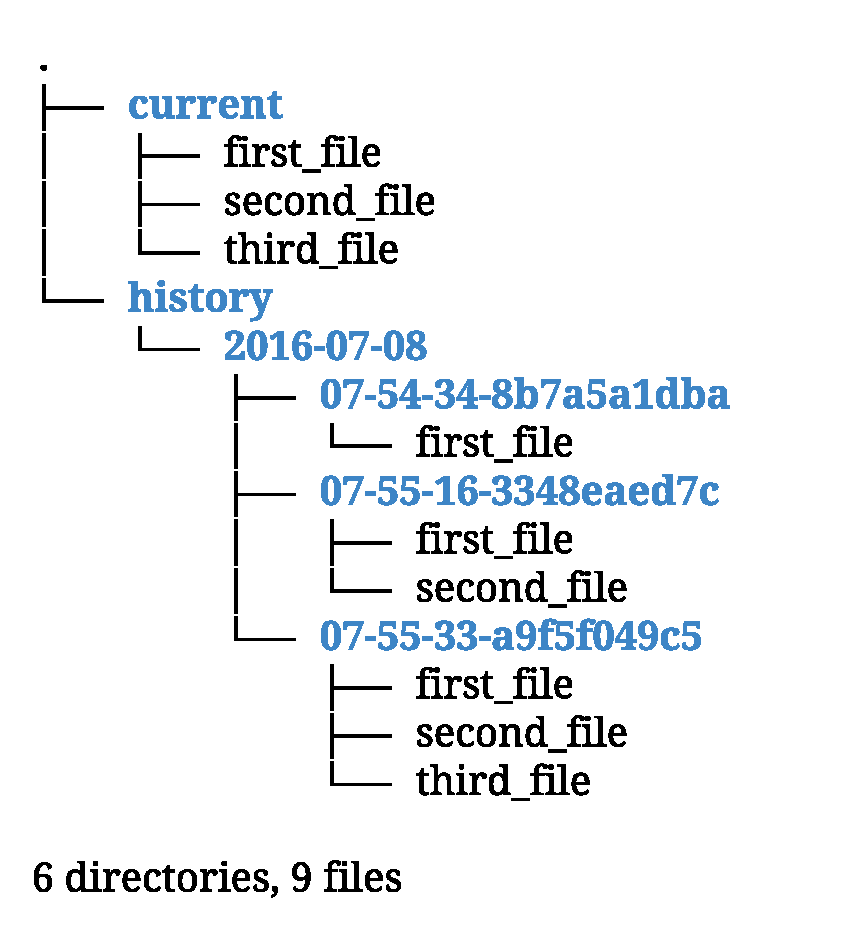
\includegraphics[width=.5\textwidth]{layout/layout}
    \caption{\label{fig:gitfslayout} Gitfs directories layout}
  \end{center}
\end{figure}

The current and history directories, showed in ~\ref{fig:gitfslayout}, are virtual directories which do not exists on disk. The entire set of operations which is done on the current directory is actually performed on the locally cloned repository. Also, in history directory, all those directories are not physical on the storage device. Those directories are created from git objects of local repository. Those objects are only once loaded in memory and cached, and from them, whenever one uses history directory or one of its directories, the content located in those is generated dynamically from the cached git objects.

\section{Views}
In order to better explain how Gitfs manages the content in those directories and the file system's operations, we can make a parallel example with how a HTTP service handles the requests.

The entire file system layout can be translated into URLs. Each path in the file system can be viewed as an URL, being part of an HTTP service. When a request is made on a certain URL, a handler will be trigger and a response will be returned. The request can be made with different HTTP (Hypertext Transfer Protocol) methods: GET, POST, PUT, DELETE etc \cite{Fielding1999}. For each of those methods the request handler can respond with different content. When a client requests the content from a certain URL it will use GET. When he wants to change it, it usually uses POST, but in order to differentiate the type of the change, other methods can be used (PUT, DELETE or PATCH). The request handler can act like a proxy and send it to other parts of the application. These get to do the actual work and return a response to the request handler which will return it back to the client.

Those parts of the application which implement the business logic are usually called controllers, in a MVC (Model View Controller) framework \cite{Deacon2009}. Other parts from a MVC framework are: Model (contains logic which deals with data manipulation) and Views (those components are what the client actually see). Traditionally, the Controller serves as a proxy for data, from Model to View. In a modern MVC architecture the business logic can be placed in an intermediary layer, between Models and Controllers, or directly in Models. Having multiple controllers, the request handler needs to decide which controller to instantiate and use, for which URL. A solution to this problem will be to route the request using some predefined routing rules. Those rules can be described using regular expressions. Because the job of a request handler is to route the request to a controller, we'll be calling it Router.

\begin{figure}[h]
  \begin{center}
    \def\svgwidth{\columnwidth}
    \input{layout/mvc.pdf_tex}
    \caption{Http routing in a MVC framework.}
    \label{fig:mvc}
  \end{center}
\end{figure}

In figure ~\ref{fig:mvc} the routing mechanism in a web MVC framework can be observed.

As one can observe, this behaviour can be applied very easily to a FUSE based file system. In order to develop a FUSE file system one needs to implement an interface that represents the set of operations which can be performed on that file system. To be more specific, fusepy offers you a base class, called 'Operations', that acts like an interface (but in Python, being weakly typed, it doesn't provide the concept of interfaces). You need to inherit from that class and implement a set of methods that represent the set of operations supported by a file system (read, write, open, close, mkdir etc.).

Because all of those methods will have a pathname as on of the arguments, we can use the model described earlier, inspired by the MVC pattern. The paths to different files or directories can be viewed as URLs and the operation as an HTTP request. We can implement different controllers for different paths and use a router to route a certain operation to a controller.

This idea came originally from Django (a popular Python based web framework \cite{Django}) which implements a variation of MVC called MVT (Model-View-Template). In this pattern, the View actually represents the controller and the Template will be the View (a little bit confusing). That's why, in our implementation, the Views are actually Controllers.

For each directory from the mount point we have implemented a series of views: CommitView, HistoryView, IndexView and CurrentView. In order to reuse the common logic of those views, we have created two classes:

\begin{itemize}
    \item PassthroughView - a view that doesn't change the behaviour of the file system. It's implemented as a blind proxy to the actual kernel file system by calling, for each operation, the corresponding system call.
    \item ReadOnlyView - used to restrict the access to any write operation. If a user space application wants to invoke a write operation, an EROFS \cite{erofs} will be raised.
\end{itemize}

Those views are inherited by the actual user facing views:
\begin{itemize}
    \item PassthroughView
    \begin{itemize}
        \item CurrentView – is the view that handles the current directory. It is a PassthroughView meaning that all operations will be executed by an individual file system, without changing the outcome. This view is also responsible for managing the changes and initiate the commit process.
    \end{itemize}

    \item ReadOnlyView
    \begin{itemize}
        \item HistoryView – view which handles the history directory and group commits by day. Also, it handles the history/{day} directories. Using the git objects from the previously cloned repository, it can retrieve commits and, using a hashmap, it will group them by day.
        \item CommitView – is the view which handles the history/{day}/{commit} directories. In a such form, a given directory represents a snapshot of the repository, when a certain change was made, in a certain day. This kind of structure is used to retrieve content, from an earlier version. It does that in a more tangible way, without the help of any commands. CommitView is read-only because you are not allowed to change the history. In order to restore a file to an older state, you need to copy it from one of those kind of directories and put it in the current directory.
        \item IndexView – is the view which handles the directory that represents the mount point. It's responsible only by current and history directory and doesn't implement any custom logic.
    \end{itemize}
\end{itemize}

All those views inherit from a base class called View. The View class has the purpose of mixing the Operations and LogginMixin classes from fusepy. Beside that, it also offer an easy mechanism for attributes initialization. See figure ~\ref{fig:views_diagram} for a better overview of the architecture.

\begin{figure}[h]
  \begin{center}
    \def\svgwidth{\columnwidth}
    \input{layout/views.pdf_tex}
  \end{center}
  \caption{Views class diagram}
  \label{fig:views_diagram}
\end{figure}

There is one special component which is not in figure ~\ref{fig:views_diagram}. That component is the Router. In order to implement the routing logic, we need a class which will look a lot like a view. Event if the Router has almost all components of a View, it can't be considered a view, because its purpose is not to implement any file system specific logic, but to act like a proxy for those components which implement.

The Router is the entry point for our file system. When mounting the file system, fusepy will receive as an argument an Operation based class. The Operation class, from fusepy, has some methods which need to be implemented in order to associate a specific behaviour to the file system. In our case, the Route doesn't need to do that, it only needs to pretend that will implement the method, but under the hood it will use the methods from specific views.

After the mounting operation is complete, FUSE kernel module, will take care of the operations. For each system call, invoked by an user space application, it will spawn a thread in which will use the object passed to it at mounting and try to call the method which implements the requested operation. Python, being a dynamic and weak typed language, we can intercept this call and inject some custom logic.

The router receive what operation needs to execute and a path to a certain file. Based on some given regular expression, it determines which view to use. Instead of initializing a new view for each operation, a cache is used. In that cache are stored initialized views, one for each file path that was requested. The cache is implemented as an LRU cache \cite{lru} in order have a hard limit on the quantity of memory used by Gitfs. The router will search in that cache, based on a cache key composed by the path of the file, and if the path is in cache, it will return the view associated to it, otherwise it will create a new one and store it in the cache.

Once the view is obtain, the Router will call the specific method which corresponds to the requested operation. A complete example is illustrated in figure ~\ref{fig:routing}.

\begin{figure}[h]
  \begin{center}
    \def\svgwidth{\columnwidth}
    \input{layout/router.pdf_tex}
  \end{center}
  \caption{Operation call flow}
  \label{fig:routing}
\end{figure}

As you can see from the example, when a read system call is used by a user space application, FUSE will trigger a read operation call, using the Router for that. The Router will check if the path is not in the cache. If not, based on regular expressions, will choose to use the CommitView, because the path to the requested file contains a full snapshot description. The Router will also pass some important information to the view, like the name of the requested file and the commit hashed, processed from the path. With those information, the CommitView will be able to retrieve the content for the `Readme.md` file, from the given date.

A common behaviour is to access the history directory, in order to see the content of a snapshot. In order to list all those directories, grouped by date and commit can lead to serious performance issues. This operations requires the git objects, in order to extract the desired content. Those git objects are on the actual disk, in the cloned repository. To avoid accessing the disk for each directory listing, we implemented an object cache in which we load all those objects once, when the file system is mounted, and every newly initialized view will be able to access them. To keep the cache consistent with repository's changes, it is invalidate at each commit and synchronization task. This process will be described later in this paper.

\section{Concurrency model and behaviour}
In order to offer a better overview of the synchronization mechanism, a presentation of the actual concurrency model is required.

As we have discussed earlier in this paper, FUSE will spawn, for each operation, a thread. This is very useful because the user can open multiple files in the same time or write onto multiple files in the same time. Another reason would be that it makes the synchronization problem much easier to solve, given the fact that those threads share the same memory. In this situation, we can share between all the threads managed by FUSE, data structures which can lock different tasks or pass information between threads.

Another interesting fact is that a FUSE based file system is a self contain process, running in user space. After the file system was mounted, a process was spawned, representing the entire application. This means, that beside the FUSE threads which share the same memory, each thread spawned by this process will share the same memory between them and between the FUSE threads' memory. Because of that, the synchronization mechanism can be decoupled by the views and router.

To keep things simple and easier, two threads, a queue and a series of locks are being used. We have named those threads workers because they are responsible for the heavy work involved in the synchronization mechanism.

All workers inherit the Peasant class which is nothing more than a specialized Thread with custom logging support.
\begin{itemize}
    \item FetchWorker - fetches changes from remote repository with a configurable frequency (the option at mount is fetch\_timeout, by default seted to 30 seconds). Between FetchWorker and SyncWorker a lock is shared in order to insure that only one fetch process is executed, at a certain point in time. The period between fetches can be configurable, by default being of 30 seconds.
    \item SyncWorker - is responsible with commit creation, merging local changes with the remote ones and pushing those changes to the remote repository. If any of these operations fail, the file system will be locked into a read-only state in order to prevent any data inconsistency problems.
\end{itemize}

Between the SyncWorker and FUSE threads are shared multiple data structure. A very important one is the job queue. After each successful change created by any CurrentView, a commit job is put on the queue. In the same time, multiple jobs can arrive on the queue. Those jobs are consumed by the SyncWorker.

For now, a CurrentView will just mark a file as being dirty and ready to be added to a commit, but will handle any commit creation responsability to the SyncWorker. The SyncWorker will aggregate those jobs and if no more commit jobs are being receive, for a given period of time (specified by 'merge\_timeout' at mount, with a default of 5 seconds) it will try to start the synchronization process.

CurrentView instances and the SyncWorker share another useful data structure, under the form of an int. It's an atomic long, with the implementation in C and with bindings in Python. This atomic long is used to keep track of how many files are still open for write or are writing. The tracking part is done by CurrentView which will increment this long each time a write operation will occur (write, chmod, chown, mkdir, rm etc.) and will decrement it when the operation was successfully finished.

The SyncWorker will check for any running write operation, using the data structure described above, and if there are still write operations, even if the merge\_timeout has expired, it will wait as many cycles until all write operations are done and all files are closed. Using this mechanism will prevent any failing in merging  and further in synchronization process.

If there is no any file open for write or any on going write operation, the SyncWorker will first try to make a commit. It can receive multiple jobs commits, each of which represents on successful change done by a CurrentView instance. Those jobs contains the file which was change, the path to it and the type of the change. In order to compose a meaningful message for the commit, it will try to understand the changes. If there is only one change it will create messages of form "Deleted <path to file>", "Deleted directory <path to directory>", "Created the <path to directory> directory", "Chmod to <mode> on <path to file>", "Rename <old file> to <new file>", "Create symbolic link to <link name> for <target>" and "Update <path to file>".

Those kind of messages are used only when a commit is compose of only one commit jobs. Otherwise, to understand what type of change was made, is more complicated and for now it uses a message of form "Update n items", where n is the number of files or directories which were updated (created, changed or removed).
After the commit was created, the SyncWorker will invalidate the commits cache for all views, forcing them to get newly created commit.

Now that the commit was created, it needed to be pushed to the remote repository as fast as possible. In order to make the process as safe as possible, the SyncWorker need to merge any existing remote changes with the local ones. In order to do that, it relies on the FetchWorker to retrieve remote changes. In the beginning of the process, the SyncWorker will set a lock on all FUSE threads in order to delay any write operation. In this way, the merge process is safe, insuring a clean staging area. Usually, the delay is not very much, depending on what kind of changes the SyncWorker needs to sync, being almost unnoticeable by the normal user (around 1-2 seconds), using a relatively small dataset of changes (<= 50 MB). Also, all fetches are stopped in order to avoid merging and race condition errors.

The SyncWorker will check it is ahead or behind. Having a commit created locally it surely is ahead, but it also can be behind if someone pushed other changes to the remote. Being behind, it means that a merge needs to be done, in order to apply the local changes over the remote ones. The merging strategy will be presented more detailed later in this paper. If the merge fails, it will try 4 more times to do the synchronization process. If it still could not merge and push, an exception will be logged and manual intervention will be needed.

Before merging to start, another fetch is being made, in order to avoid not having all remote changes in the local repository (otherwise, it could lead to push errors and a retry should processed). In case of a successful merge, will try to push the changes on the remote repository. In case of failing, it will retry it after another cycle of timeout, restarting the synchronization process.

After a sync has been complete, write operations will be free to execute. Also, the fetches will start again.

This process can start even if there is no commit to create. The SyncWorker works in cycles with the period defined by merge\_timeout (default to 5 seconds). If there was no activity on the file system, it will start the synchronization process in order to bring in the current directory any change which was pushed to the remote repository by a different system. If there are in progress write operations and remote changes which needed to be synced, the SyncWorker will wait until all write operations are finished and files are closes.

\begin{figure}[h]
  \begin{center}
    \def\svgwidth{\columnwidth}
    \input{layout/concurrency_model.pdf_tex}
  \end{center}
  \caption{Concurrency model of Gitfs}
  \label{fig:concurrency}
\end{figure}

In figure ~\ref{fig:concurrency} are all components involved in the synchronization process.

If any errors will occur in this process, will merging, pushing or fetching, the file system will enter in read-only mode. In this mode any change operations are denied. This is a safe mechanism to ensure that no data is corrupted and that the repository will stay in a state from which will be possible to make it functional. In case of failure (network, human or simple bug), the SyncWorker will retry to sync the changes, using a total of 5 attempts. If there is no success after those, the human intervention is mandatory, otherwise the file system will remain in read-only mode.

Because running multiple Gitfs, each having the same server as origin (with different repositories), could lead to a network flood when multiple FetchWorkers will fetch in the same time and given the fact that if a user is not using the file system, doing fetches in the background means wasting resource, the idle mode was introduced. If Gitfs enters in this mode it will lower down the fetches frequency, changing the period between fetches to 30 minutes (given by idle\_fetch\_timeout which can be overridden at mount).

This idle mode is triggered after no operation was triggered by FUSE, meaning no active user is using the file system, for more than a given amount of time. This amount of time is given by the SyncWorker and represents the number of cycles that need to pass in order to switch to idle mode. This number is a configurable one and can be overridden at mount (min\_idle\_times, by default to 10). Given the fact that the default period of a cycle is 5 seconds, the idle mode will be on after 50 seconds of inactivity on the file system.

\section{Merging}

Earlier in this paper we discussed about merging remote changes with local changes. Gitfs uses a strategy called always-accept-mine. This strategy is the only one implemented right now, but the merging strategy component is implemented in an extensible manner.

\begin{figure}[h]
  \begin{center}
    \def\svgwidth{\columnwidth}
    \input{layout/commits.pdf_tex}
  \end{center}
  \caption{Diverging commits}
  \label{fig:commits}
\end{figure}

We will use the situation represented in ~\ref{fig:commits} as an example for this strategy. In figure ~\ref{fig:commits} there are two branches represented, called remote and local, which have a common branch. On that common branch, commits 1, 2 and 3 will be present on local and remote branch. From commit 3, those branches start diverging. On branch remote commits 4, 5, 6 are created and on local, commits 7 and 8.

The plan is to apply local changes over the remote ones, obtaining a nice chain of commits: 1, 2, 3, 4, 5, 6, 7' and 8'. In order to obtain that we need to know which was the diverging commit or the common parent.

For that we'll use very simple algorithm and two sets, one for each branch. We'll start from the end and the last commits of those branches. Each retrieved commit will be put in the corresponding set, but first we'll do a cross checking. We'll check to see if the commit from the first branch is already in the set of commits for the second branch. The same will be done for the commit of the second branch. If we find any commit in other branches lists, then we can stop, we found the parent.

In our example, we pick commit 6, from branch remote, and check to see if it's present in the set of commits for branch local . It's the first commit so this is not the case. We add it to the list of visited commits. Now we pick 8, from branch local, and check to see if is not already in the set of remote's  visited commits.
Only 6 is present so we'll add 8 in the set of local's visited commits. We'll continue to do the same for 5 and 7, 4 and 3. Now 3 is in the set of local's visited commits. Next we'll be comparing 3 and 2. 3 is already in a set so we can stop, because we found the last common commit.

This algorithm is a very simple one, in which we rely on the set data structure which offers us an $O(1)$ lookup complexity. Worst case time complexity, for this algorithm, is $O(n)$, where $n$ represents the number of commits in a branch. In normal usage parameters, the number of diverging commits is very small, around 10-20.

Now that we found the last common commit, we'll rename the branches in merging\_remote and merging\_local in order to avoid braking up the local repository. We switch to merging\_remote and use this branch as the active, working one. From merging\_local we'll take the commits proceeding the common one and we'll try to merge them on top of merging\_remote.

If one want to use another strategy, it needs to implement it by creating a class which inherits from the base strategy (which is locate in the mergers module) and has a method called merge. That method will be called with a reference to the local branch, on to the remote branch and a reference to the remote repository. After the code base is merged and a new build is released, the newly created strategy can be used. We'll be using Libgit2 for merging, which will try to merge the commits by using a 3 way merge strategy. If it fails, we'll need to handle it manually.

In case of conflicts, Libgit2 will return a data structure which will help us solved them easily. There are three types of conflicts which this strategy knows to resolve:
\begin{itemize}
    \item delete by us, but not by them. In this case we'll be deleting the file.
    \item delete by them, but not by us. In this case we'll be adding back the file.
    \item both changed the file. In this case we'll be overwriting the file with the content from our local repository. Is not the best approach because it can override already merged changes.
\end{itemize}

After each merge with conflict, a new commit is created, having the same meta data as the local commit which was merged.

\begin{figure}[h]
  \begin{center}
    \def\svgwidth{\columnwidth}
    \input{layout/merging-end.pdf_tex}
  \end{center}
  \caption{Branch layout after merging}
  \label{fig:merging}
\end{figure}

In figure ~\ref{fig:merging} you can see which and how the commits are being applied. Finally, we'll rename the merging\_remote branch in local and remove the merging\_local branch. In this way, the repository is not polluted with unused branches.

In case of exceptions, we'll be reverting to the local branch and remove any reference to merging\_local and merging\_remote.

Always-accept-mine strategy is a strategy in which local changes will be more important than remote ones. In this strategy, if a conflict is detected within a file, with changes coming from remote and local, the conflict will be solved by replacing its entire content with local content of the file.

\section{Tests}

A file system is an important part of a system. If the file system fails, other components may fail. Because of that, Gitfs has a large suite of tests, from integration to unit tests. Besides the components exposed in this paper, Gitfs has more utility components and data structure that need to be tested.

Testing a file system could seem easy at a first glance. If a user space application creates a file, that file should be on the disk and accessible by another user space application. In the context of Gitfs, the entire synchronization flow needs to be tested, in order to see if earlier created changes have arrived on the remote.

To replicate the testing environment as closely as possible to the general setup and to be easy to reproduce this environment, Gitfs uses privileged Docker containers \cite{Merkel2014}. The entire environment is build using make rules and can be replicated in any testing setup (host, virtual machine or Linux containers \cite{Rosen2014}). On the official repository, Gitfs is tested automatically whenever a new change is pushed to it. The Drone CI \cite{Drone2016} is a continuous integration system that integrates with Github which, for every git push, will trigger a job drone. Drone is open source and configurable. Each git repository contains a .drone.yml file (having YAML format \cite{Ben-Kiki2009}), in which descriptive instructions are given to drone about the environment. Those instructions are very different starting from which Docker image to use as base environment to what testing command to use and what to do after the testing in case of success or fail.

In figure ~\ref{fig:pipeline} the entire development pipeline is described.

\begin{figure}[h]
  \begin{center}
    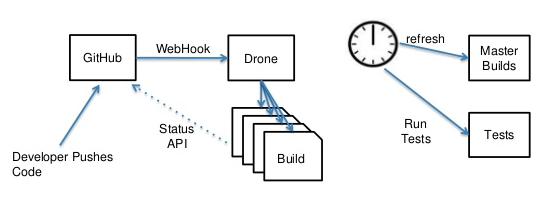
\includegraphics[width=\textwidth]{layout/drone.png}
  \end{center}
  \caption{Gitfs development pipeline \cite{GDR}}
  \label{fig:pipeline}
\end{figure}

The testing environment contains a bare git repository, its local clone with initial files, directories and commits, and a directory which serves as the mount point. When the testing process begins, the environment is created by different make rules \cite{Aham-cumming2015}, followed by other make rules in order to run the tests collection. In the end, another make rule will be applied in order to clean the environment.

In this moment, Gitfs has 222 tests which offer a 92\% coverage. The coverage percentage comes from unit tests, and doesn't reflect the true coverage \cite{Inozemtseva2014}. In order to assure a better testing coverage, rigours integration tests are needed. In Gitfs every operations which an user space application can perform on a POSIX complaint file system is tested, ensuring the fact that Gitfs is a POSIX complaint file system. Beside those operations, the concurrency model is tested by simulating the collaboration part.

An usual test looks like this: once the environment is created and the file system mounted, we use an user space application to write content to a newly created file. We close the file and check to see that the content is there. We wait until Gitfs is doing the synchronization process. In another locally cloned repository, we fetch the changes which were supposed to be pushed by Gitfs. Finally we checked if the fetched changes are the ones which were made through the user space application. The entire process can be slow, but we are using a custom configured Gitfs instance, in which we set the merge\_timeout and fetch\_timeout as low as possible (100 milliseconds). Another trick that we use was not to wait an empiric amount of time until we thought that the process will be finished, but to use a custom log parser, which will analyse and block the execution of tests until a certain log message will be created by the SyncWorker and the FetchWorker.

\section{Configurable Options}
In chapters above we also presented different configurable options. Gitfs has more options which can be found below. Those options will be passed to Gitfs in the mounting process, using the -o argument of mount command. Multiple Gitfs options need to be concatenated and split by a comma (-o option1=value1,option2=value2...).

\begin{itemize}
    \item remote\_url: the URL of the remote repository
    \item branch: the branch name to follow (default: master)
    \item repo\_path: the location where the repository will be cloned and used by Gitfs
    (default: $/var/lib/gitfs/repo\_path$)
    \item max\_size: the maximum file size in MBs allowed for an individual file. If set to 0, then allow any file size (default: 10MB)
    \item user: the user that will mount the file system (default: root)
    \item group: the group that will mount the file system (default: root)
    \item committer\_name: the name that will be displayed for all the commits (default: user)
    \item committer\_email: the email that will be displayed for all the commits (default: user@FQDN)
    \item merge\_timeout: the interval between idle state and commits/pushes (default: 5s)
    \item fetch\_timeout: the interval between fetches (default: 30s)
    \item log: the path of the log file. Special name syslog will log to the system logger (default: syslog)
    \item log\_level: the logging level. One of error, warning, info, debug (default: warning)
    \item debug: he switch that sets the log level to debug and also enables FUSE’s debug (default: false)
    \item username: the username for HTTP basic auth
    \item password: the password for HTTP basic auth
    \item key: the path of the SSH private key. NOTE: the public key is constructed by appending .pub to this path and the file MUST exist (default: \textdollar HOME/.ssh/id\_rsa)
\end{itemize}
